\subsection{UC 9 - Creazione condivisione evento} \label{sec:UC9}

    \begin{itemize}
        \item \textbf{Attore principale}: MUA;
        \item \textbf{Descrizione}: il MUA invia le informazioni dell'evento da condividere al sistema;
        \item \textbf{Precondizioni}: il MUA sta usando la funzionalità di creazione di una condivisione;
        \item \textbf{Postcondizioni}: il sistema condivide l'evento con l'indirizzo e-mail fornito dal MUA;
        \item \textbf{Scenario principale}:
            \begin{enumerate}
                \item il MUA trasmette l'id dell'evento da condividere (\hyperref[sec:UC9.1]{UC 9.1});
                \item il MUA trasmette l'indirizzo e-mail a cui condividere (\hyperref[sec:UC9.2]{UC 9.2});
                \item il sistema condivide l'evento;
            \end{enumerate}
        \item \textbf{Inclusioni}: nessuna;
        \item \textbf{Generalizzazioni}: nessuna;
        \item \textbf{Estensioni}: nessuna.
    \end{itemize}

    \begin{figure}[H]
        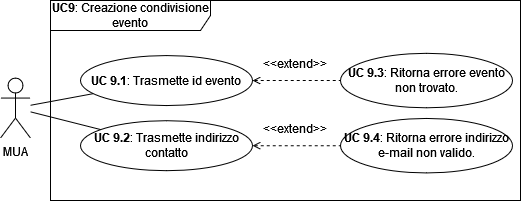
\includegraphics[width=0.85\textwidth]{sections/uc_imgs/UC09.png}
        \centering
        \caption{Diagramma sotto-casi UC 9}
    \end{figure}

    \subsubsection{UC 9.1 - Trasmette id evento} \label{sec:UC9.1}
    \begin{itemize}
        \item \textbf{Attore principale}: MUA;
        \item \textbf{Descrizione}: il MUA trasmette l'id dell'evento per condividere l'evento;
        \item \textbf{Precondizioni}: il MUA sta usando la funzionalità di creazione condivisione di un evento;
        \item \textbf{Postcondizioni}: il sistema conosce l'id dell'evento da condividere;
        \item \textbf{Scenario principale}:
            \begin{enumerate}
                \item il MUA invia l'id dell'evento per condividerlo;
            \end{enumerate}
        \item \textbf{Inclusioni}: nessuna;
        \item \textbf{Generalizzazioni}: nessuna;
        \item \textbf{Estensioni}:
            \begin{enumerate}[label=\alph*.]
                \item il sistema non riesce a condividere l'evento perché l'id dell'evento fornito non è stato trovato:
                \begin{enumerate}[label=\arabic*.]
                    \item il sistema ritorna un errore al MUA di evento non trovato (\hyperref[sec:UC9.3]{UC 9.3}).
                \end{enumerate}
            \end{enumerate}
    \end{itemize}


    \subsubsection{UC 9.2 - Trasmette l'indirizzo e-mail} \label{sec:UC9.2}
    \begin{itemize}
        \item \textbf{Attore principale}: MUA;
        \item \textbf{Descrizione}: il MUA trasmette l'indirizzo e-mail per la condivisione al sistema;
        \item \textbf{Precondizioni}: il MUA sta usando la funzionalità di creazione condivisione di un evento;
        \item \textbf{Postcondizioni}: il sistema conosce l'indirizzo e-mail a cui condividere;
        \item \textbf{Scenario principale}:
            \begin{enumerate}
                \item il MUA invia l'indirizzo e-mail per la condivisione al sistema;
                \item il sistema controlla che le informazioni ricevute rispettino il seguente requisito minimo:
                    \begin{itemize}
                        \item l'indirizzo email del contatto non è una stringa vuota;
                    \end{itemize}
            \end{enumerate}
        \item \textbf{Inclusioni}: nessuna;
        \item \textbf{Generalizzazioni}: nessuna;
        \item \textbf{Estensioni}:
            \begin{enumerate}[label=\alph*.]
                \item il sistema non riesce a creare la condivisione dell'evento perché l'indirizzo e-mail fornito non è valido:
                \begin{enumerate}[label=\arabic*.]
                    \item il sistema ritorna un errore al MUA di indirizzo e-mail non valido (\hyperref[sec:UC9.4]{UC 9.4}).
                \end{enumerate}
            \end{enumerate}
    \end{itemize}


\subsubsection{UC 9.3 - Ritorna errore evento non trovato} \label{sec:UC9.3}
    \begin{itemize}
        \item \textbf{Attore principale}: MUA;
        \item \textbf{Descrizione}: il sistema non riesce a condividere l'evento perché l'evento non è stato trovato;
        \item \textbf{Precondizioni}: il MUA ha inviato l'id dell'evento da condividere;
        \item \textbf{Postcondizioni}: il sistema non condivide l'evento, il MUA è stato notificato dell'errore;
        \item \textbf{Scenario principale}:
            \begin{enumerate}
                \item il sistema non trova l'evento con l'identificativo fornito dal MUA;
                \item il sistema non condivide l'evento e notifica il MUA dell'errore;
            \end{enumerate}
        \item \textbf{Inclusioni}: nessuna;
        \item \textbf{Generalizzazioni}: nessuna;
        \item \textbf{Estensioni}: nessuna.
    \end{itemize}

    \subsubsection{UC 9.4 - Ritorna errore indirizzo e-mail non valido} \label{sec:UC9.4}
    \begin{itemize}
        \item \textbf{Attore principale}: MUA;
        \item \textbf{Descrizione}: il sistema non riesce a condividere l'evento perché l'indirizzo e-mail del contatto non rispetta i requisiti;
        \item \textbf{Precondizioni}: il MUA ha inviato l'indirizzo e-mail a cui condividere;
        \item \textbf{Postcondizioni}: il sistema non condivide l'evento, il MUA è stato notificato dell'errore;
        \item \textbf{Scenario principale}:
            \begin{enumerate}
                \item il sistema controlla la sintassi dell'indirizzo e-mail e trova un errore;
                \item il sistema non condivide l'evento e notifica il MUA dell'errore;
            \end{enumerate}
        \item \textbf{Inclusioni}: nessuna;
        \item \textbf{Generalizzazioni}: nessuna;
        \item \textbf{Estensioni}: nessuna.
    \end{itemize}
